% parameters for the MPS drawings
\definecolor{Tcolor}{RGB}{255, 235, 171}
\definecolor{Wcolor}{RGB}{190, 190, 255}
\def\textoffsetVertical{0.8}
\def\nodewidth{0.6cm}
\def\legwidth{0.8}
\def\nodedistance{1.5}
\def\textoffsetVerticalW{0.9}
\def\textoffsetHorizontalW{-0.9}
\def\textoffsetVerticalMPO{1.2}
\def\yoffset{1}
\def\xoffset{3}
\def\resultMPSYoffset{2.5}
\def\resultMPSXOffsetSmall{2}
\def\resultMPSXOffset{3}
\def\dotsOffset{3}
\def\conjOffsetVertical{1.5}
\def\conjOffsetVerticalLarge{2.2}
%
One of the main problems concerning quantum systems is time evolution. The goal is to find the
state at a time $t$, under the condition that the state at time $t_0$ is known and the time-dependent Schrödinger equation
\begin{equation*}
    \frac{d}{dt}\ket*{\Psi(t)} = -i\hat{H}(t)\ket*{\Psi(t)}
\end{equation*} 
holds, where we have set $\hbar = 1$. There exist many algorithms implementing time evolution directly on MPS \cite{Paeckel:2019}. 
Some of these algorithms, for example the very popular Time Evolving Block Decimation (TEBD \cite{Website:TEBD}), are not applicable to long-range interactions.
Here, we will focus on two methods in particular, the fourth order Runge Kutta method (RK4) and the Time Dependent Variational Principle (TDVP), which work with a Hamiltonian given as an MPO and can handle long-range interactions.
Implementations of both methods can be found at \cite{Sappler:2023}.

\subsection{Runge-Kutta}
The fourth order Runge-Kutta or RK4 method is a well known numerical method for solving linear equations.
With this method, the state at time $t + \Delta t$ can be computed from the state at time $t$ as
\begin{equation*}
    \ket*{\Psi(t+\Delta t)} \approx \ket*{\Psi(t)} + \frac{\Delta t}{6}\big(
        \ket*{k_1} + 2\ket*{k_2} + 2\ket*{k_3} + \ket*{k_4}
    \big),
\end{equation*}
where
\begin{equation*}
    \begin{split}
        \ket*{k_1} &= -i\hat{H}\left(t\right)\ket*{\Psi(t)}, \\
        \ket*{k_2} &= -i\hat{H}\left(t + \Delta t/2\right)\left(\ket*{\Psi(t)} + \frac{\Delta t}{2}\ket*{k_1}\right), \\
        \ket*{k_3} &= -i\hat{H}\left(t + \Delta t/2\right)\left(\ket*{\Psi(t)} + \frac{\Delta t}{2}\ket*{k_2}\right), \\
        \ket*{k_4} &= -i\hat{H}\left(t + \Delta t\right)\left(\ket*{\Psi(t)} + \Delta t\ket*{k_3}\right).
    \end{split}
\end{equation*}
For this method to work with MPSs and MPOs we have to implement two operations: Addition of two MPSs and multiplication of an MPS with an MPO.
The addition of two MPSs
\begin{equation*}
    \ket*{\Psi} = \sum_{l_1, l_2, \dots, l_N} \trace\left(
        \vectorbold{A}^{[1],l_1} \vectorbold{A}^{[2],l_2} \cdots \vectorbold{A}^{[N],l_N}
    \right) \ket*{l_1, l_2, \dots, l_N}
\end{equation*}
and
\begin{equation*}
    \ket*{\Phi} = \sum_{l_1, l_2, \dots, l_N} \trace\left(
        \vectorbold{B}^{[1],l_1} \vectorbold{B}^{[2],l_2} \cdots \vectorbold{B}^{[N],l_N}
    \right) \ket*{l_1, l_2, \dots, l_N}
\end{equation*}
can be constructed by merging the tensors for each sub system block diagonally \cite{Weitang:2020}:
\begin{equation*}
    \begin{split}
        \ket*{\Psi} + \ket*{\Phi} &= \sum_{l_1, l_2, \dots, l_N} \trace\left(
        \vectorbold{C}^{[1],l_1} \vectorbold{C}^{[2],l_2} \cdots \vectorbold{C}^{[N],l_N}
    \right) \ket*{l_1, l_2, \dots, l_N}, \\
    \vectorbold{C}^{[n], l_n} &= \begin{pmatrix}
        \vectorbold{A}^{[n], l_n} & \vectorbold{0}              \\
        \vectorbold{0}            & \vectorbold{B}^{[n], l_n}
    \end{pmatrix}.
    \end{split}
\end{equation*}
If the bond dimensions of the original two MPSs are $\chi_1$ and $\chi_2$, the resulting MPS has bond dimension $\chi_1 + \chi_2$. \\
Applying an MPO to an MPS can be done by contracting the two networks together along their physical legs. The result of applying
the MPO (\ref{eq:mpo}) to the MPS (\ref{eq:mps}) is
\begin{equation*}
    \begin{split}
        \hat{H}\ket*{\Psi} = \sum_{l_1, l_2, \dots, l_N} \trace\left(
            \vectorbold{D}^{[1],l_1} \vectorbold{D}^{[2],l_2} \cdots \vectorbold{D}^{[N],l_N}
        \right) \ket*{l_1, l_2, \dots, l_N}, \\
        D^{[n],l_n}_{k_{n-1},k_n} \coloneqq D^{[n],l_n}_{(i_{n-1}j_{n-1}),(i_nj_n)} = \text{reshape}\left(
            \sum_{l_n^\prime} W^{[n],l_n,l_n^\prime}_{j_{n-1},j_n} A^{[n],l_n^\prime}_{i_{n-1},j_n}
            \right),
    \end{split}
\end{equation*}
where the tensors $\vectorbold{C^{[n]}}$ are computed by first contracting the $A^{[n]}$ and $W^{[n]}$ tensors along their physical
legs and then reshaping the result, grouping together the virtual legs $i_{n-1}$ with $j_{n-1}$ and $i_n$ with $j_n$. 
The operation can also be written diagrammatically:
\begin{equation*}
    \vcenter{\hbox{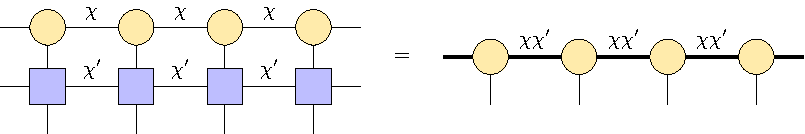
\includegraphics[]{figures/tikz/mps/basic/applying_mpo_to_mps.pdf}}}.
\end{equation*}
\noindent Applying an MPO to an MPS also increases the bond dimension: If the bond dimension of the original MPS is $\chi$
and the bond dimension of the MPO is $\chi^\prime$, the bond dimension of the result will be $\chi\cdot\chi^\prime$. \\
\noindent We have seen that both the addition of two MPSs and the multiplication of an MPS with an MPO increase the bond dimension.
This is a problem since the computational cost of both operations scales with a power of the bond dimension.
Therefore we need to truncate the MPS regularly. This can for example be done by sweeping accross the MPS, performing singular value decompositions,
and keeping only the $N_\text{trunc}$ largest singular values \cite{Weitang:2020}.

\subsection{Time Dependent Variational Principle (TDVP)}
The idea of the Time Dependent Variational Principle \cite{Vanderstraeten:2019,Haegeman:2016,Website:TDVP} is to project the right hand side of the Schrödinger equation to the \textit{tangent space}
of the MPS:
\begin{equation}
    \label{eq:time_evolution_equation_TDVP}
    \frac{d}{dt}\ket*{\Psi(t)}_\text{MPS} = -i\hat{P}_{T{\ket*{\Psi(t)}_\text{MPS}}}\hat{H}(t)\ket*{\Psi(t)}_\text{MPS}.
\end{equation} 
The tangent space is a manifold of MPSs that are orthogonal to the current MPS state $\ket*{\Psi(t)}_\text{MPS}$.
When integrating this equation, the resulting state never leaves the MPS manifold. \\
There are two versions of TDVP, one that updates MPS tensors one after the other (TDVP1), and one that updates two neighbouring MPS tensors
at once (TDVP2). We will focus on TDVP2, since it allows to grow the bond dimension as needed, whereas TDVP1 assumes a fixed bond dimension. \\
To discuss the algorithm, we must first introduce the canonical form of MPSs. When constructing an MPS, we have an inherent gauge degree of freedom,
because we can replace every tensor in the MPS
\begin{equation*}
    \vcenter{\hbox{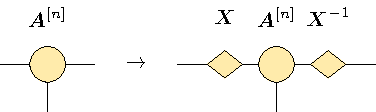
\includegraphics[]{figures/tikz/mps/tdvp/replacing_mps_tensor_with_canonical.pdf}}}
\end{equation*}
and recover the original MPS. This gauge degree of freedom can be used to transform any MPS into the \textit{mixed canonical form}
\begin{equation*}
    \vcenter{\hbox{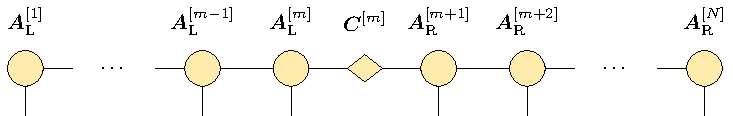
\includegraphics[]{figures/tikz/mps/tdvp/mps_in_canonical_form.pdf}}},
\end{equation*}
where it holds
\begin{equation*}
    \vcenter{\hbox{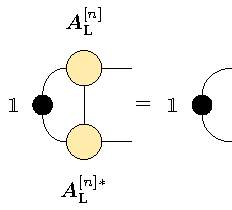
\includegraphics[]{figures/tikz/mps/tdvp/left_environment_contraction.pdf}}}, \quad\quad\quad\quad
    \vcenter{\hbox{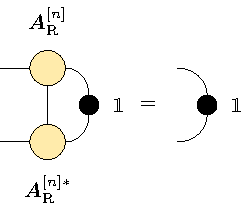
\includegraphics[]{figures/tikz/mps/tdvp/right_environment_contraction.pdf}}} \quad\quad\quad\quad \forall n\in\{1,2,\dots,N\}.
\end{equation*}
$\vb*{A}_L^{[n]}$ and $\vb*{A}_R^{[n]}$ are then called \textit{left}-/\textit{right}-\textit{canonical} and $\vb*{C^{[m]}}$ is the \textit{orthogonality center}.
Algorithms to turn any MPS into mixed canonical form and to shift the orthogonality center around can be found in \cite{Schollwöck:2011,Hauschild:2018}.\\
Assume now that the current MPS is given in mixed-canonical form. It is possible to show that the tangent space projection operator then has the form \cite{Vanderstraeten:2019,Haegeman:2016}
\begin{equation*}
    \hat{P}_{T{\ket*{\Psi(t)}_\text{MPS}}} = \sum_{n=1}^{N} \vb*{P}_\text{L}^{[1:n-1]}\otimes\mathbbm{1}^{[n]}\otimes\vb*{P}_\text{R}^{[n+1:N]}
    - \sum_{n=1}^{N-1} \vb*{P}_\text{L}^{[1:n]}\otimes\vb*{P}_\text{R}^{[n+1:N]},
\end{equation*}
where
\begin{equation*}
    \vb*{P}_\text{L}^{[1:n]}\ = 
    \vcenter{\hbox{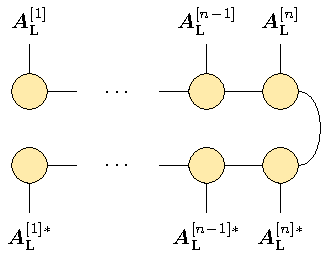
\includegraphics[]{figures/tikz/mps/tdvp/left_projector.pdf}}}
\end{equation*}
and
\begin{equation*}
    \vb*{P}_\text{R}^{[n:N]} = 
    \vcenter{\hbox{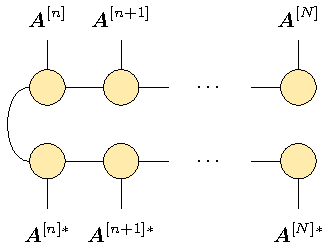
\includegraphics[]{figures/tikz/mps/tdvp/right_projector.pdf}}}.
\end{equation*}
We can now write the right hand side of the time evolution Equation (\ref{eq:time_evolution_equation_TDVP}), up to the factor $-i$, as
\begin{equation*}
    \begin{split}
        &\hat{P}_{T{\ket*{\Psi(t)}_\text{MPS}}}\hat{H}(t)\ket*{\Psi(t)}_\text{MPS}\\
        &\\
        =&\sum_{n=1}^{N} 
        \quad\vcenter{\hbox{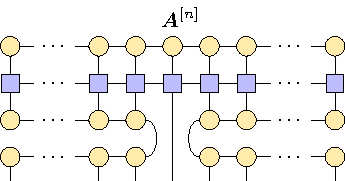
\includegraphics[]{figures/tikz/mps/tdvp/time_evolution_right_hand_side_1a.pdf}}}\quad
        -\sum_{n=1}^{N-1}
        \quad\vcenter{\hbox{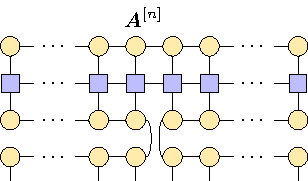
\includegraphics[]{figures/tikz/mps/tdvp/time_evolution_right_hand_side_1b.pdf}}}\quad\\
        &\\
        =& \sum_{n=1}^{N} 
        \quad\vcenter{\hbox{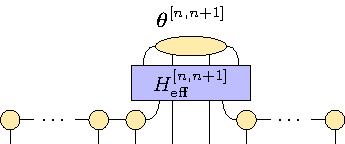
\includegraphics[]{figures/tikz/mps/tdvp/time_evolution_right_hand_side_2a.pdf}}}\quad
        -\sum_{n=1}^{N-1}
        \quad\vcenter{\hbox{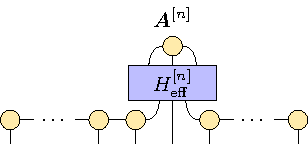
\includegraphics[]{figures/tikz/mps/tdvp/time_evolution_right_hand_side_2b.pdf}}}\quad,
        \end{split}
\end{equation*}
where we introduced the two-site tensor $\vb*{\theta}^{[n, n+1]}$, which can be constructed by contracting the two neighbouring
tensors $\vb*{A}^{[n]}$ and $\vb*{A}^{[n+1]}$. Additionally, we contracted the MPO with parts of the MPS into the
effective two-site and one-site Hamiltonians $H_\text{eff}^{[n,n+1]}$ and $H_\text{eff}^{[n]}$. \\
In the following, the TDVP2 algorithm is briefly summarized. A more in-depth description can be found at \cite{Vanderstraeten:2019,Haegeman:2016,Website:TDVP}.
The algorithm sweeps through the MPS, updating pairs of neighbouring tensors along the way. A single update on the two-site tensor $\vb*{\theta}^{[n, n+1]}$
during the process of sweeping from left to right is made as follows: 
First, we contract $\vb*{\theta}^{[n, n+1]}$ with
\begin{equation}
    \label{eq:TDVP_mat_exp_1}
     \exp\left(-\frac{i\Delta t}{2}H_\text{eff}^{[n, n+1]}\right).
\end{equation}
We then split and truncate the resulting tensor using SVD to obtain the updated tensors $\vb*{A}^{[n]\prime}$ and $\vb*{A}^{[n+1]\prime}$.
Next, we apply 
\begin{equation}
    \label{eq:TDVP_mat_exp_2}
    \exp\left(\frac{i\Delta t}{2}H_\text{eff}^{[n]}\right)
\end{equation}
to $\vb*{A}^{[n+1]\prime}$, forming $\vb*{A}^{[n+1]\prime\prime}$. Finally, we can contract 
$\vb*{A}^{[n+1]\prime\prime}$ with $\vb*{A}^{[n+2]}$ to form the two-site tensor for the next step.
We repeat this procedure until we arrive at the right-most tensor of the MPS. Sweeping from right to left can be done analogeously. \\
After sweeping through the MPS from left to right and back, we have performed a full time step $\Delta t$ and obtain the updated MPS
$\ket*{\Psi(t+\Delta t)}_\text{MPS}$.\\
The implementation of TDVP2 is very similar to the implementation of the popular DMRG algorithm \cite{Schollwöck:2011};
it is possible to obtain TDVP2 from DMRG by only changing a few lines of code \cite{Haegeman:2016}. It is worth to note that 
it is not necessary to compute the matrix exponentials (\ref{eq:TDVP_mat_exp_1}) and (\ref{eq:TDVP_mat_exp_2}) directly, which is a costly
operation. Instead, we only need the result of multiplying the matrix exponential with the current state vector $\vb*{\theta}^{[n, n+1]}$ or $\vb*{A}^{[n+1]\prime}$,
which can be computed efficiently, e.g., using the scipy function \verb|scipy.expm_multiply|. \\
An efficient implementation also involves storing environment tensors of every site in a list and updating them during a sweep,
such that the effective Hamiltonians do not have to be recomputed from scratch at each step.